\documentclass{ntuthesis}	% defined in ./ntuthesis.cls


% \usepackage{mathptmx}		% font
\usepackage{verbatim}
\usepackage{color}
\usepackage{url}
\usepackage{graphicx}
\usepackage{array}
\usepackage{wallpaper}
\usepackage{hyperref}
\usepackage{graphicx}
\usepackage{tikz}
\usepackage{physics}		% some convenient math commands, used in examples
\usepackage{lipsum} 		% dummy text 

%% font settings
%% font settings

% Chinese font
% use 標楷體 on your computer
\setCJKmainfont[AutoFakeBold=2,AutoFakeSlant=.2]{DFKai-SB} 

% English font
% see README for more information
\usepackage[T1]{fontenc}
\usepackage{textcomp}

% set text font as Times
% load before mtpro2 the for correct mathrm font
\renewcommand{\rmdefault}{ptm} 

\usepackage[lite,subscriptcorrection,slantedGreek,nofontinfo]{mtpro2}
\usepackage{bm}
\usepackage[scaled=0.92]{helvet}
 
 
% \setmainfont[Mapping=rijke]{Times New Roman}
% \setsansfont{Arial}
\setmonofont{Courier New} 
% \usepackage{unicode-math}			% specifying TNR math font
% \setmathfont{TeX Gyre Termes Math} 
 
 


%% Your information goes here
% author: Tz-Huan Huang [http://www.csie.ntu.edu.tw/~tzhuan]

% ----------------------------------------------------------------------------
% "THE CHOCOLATE-WARE LICENSE":
% Tz-Huan Huang wrote this file. As long as you retain this notice you
% can do whatever you want with this stuff. If we meet some day, and you think
% this stuff is worth it, you can buy me a chocolate in return Tz-Huan Huang
% ----------------------------------------------------------------------------

% Syntax: \var{English}{Chinese}
\university{National Taiwan University}{國立臺灣大學}
\college{College of Typesetting}{排版學院}
\institute{Department of \LaTeX \: Typesetting}{\LaTeX 排版學系}
\title{NTU Thesis Template}{台大學士/碩士/博士論文模板}
\author{English Name}{中文名字}
\studentid{B09876543}
\advisor{Ming-Zhi Name, Ph.D.}{名字 博士}
\defenseyear{2000}{89}
\defensemonth{January}{1}
\defenseday{1}
\doi{doi:10.6342/NTU2017XXXXX}
\keywords{keyword1, keyword2, keyword3}{關鍵字1、 關鍵字2、 關鍵字3}



% Using the tex-text mapping for ligatures etc.
% \defaultfontfeatures{Mapping=tex-text} % ???


\ifdefined\firstpage

  % \ifdefined\withwatermark
  %   \newsavebox\mybox
  %   \savebox\mybox{\tikz[opacity=0.5]\node{
\includegraphics{watermark.pdf}};}
  %   \newwatermark*[allpages,xpos=6.1725cm,ypos=10.5225cm,scale=0.5]{\usebox\mybox}
  % \fi

  % digital object identifier
  \ifdefined\withdoi
    \insertdoi
  \fi
\fi

%% bibliography settings
\usepackage[style=ieee,
			backend=bibtex, 
			url=false, 
			eprint=false, 
			doi=false, 
			isbn=false,
			citestyle=numeric-comp]{biblatex}		% specifying 9pt bib text
			\addbibresource{./reference.bib}  % bib path
 
% hyperlink on journal names
\ExecuteBibliographyOptions{doi=false}
\DeclareFieldFormat{doilink}{
\iffieldundef{doi}{#1}
{\href{http://dx.doi.org/\thefield{doi}}{#1}}}

\DeclareBibliographyDriver{article}{%
  \usebibmacro{bibindex}%
  \usebibmacro{begentry}%
  \usebibmacro{author/translator+others}%
  \setunit{\labelnamepunct}\newblock
  \usebibmacro{title}%
  \newunit
  \printlist{language}%
  \newunit\newblock
  \usebibmacro{byauthor}%
  \newunit\newblock
  \usebibmacro{bytranslator+others}%
  \newunit\newblock
  \printfield{version}%
  \newunit\newblock
  \usebibmacro{in:}%
  \href{http://dx.doi.org/\thefield{doi}}{%
  \usebibmacro{journal+issuetitle}%
  \newunit\newblock
  \usebibmacro{byeditor+others}%
  \newunit\newblock
  \usebibmacro{note+pages}}%
  \newunit\newblock
  \iftoggle{bbx:isbn}
   {\printfield{issn}}
   {}%
  \newunit\newblock
  \usebibmacro{doi+eprint+url}%
  \newunit\newblock
  \usebibmacro{addendum+pubstate}%
  \newunit\newblock
  \usebibmacro{pageref}%
  \usebibmacro{finentry}
  } 
 
 


%% create metadata?
\makeatletter
\AtBeginDocument{
  \hypersetup{
    pdftitle={\@titleen},
    pdfauthor={\@authoren},
    pdfsubject={\@typeen{} \@classen},
    pdfkeywords={\@keywordsen}
  }
}
\makeatother


\begin{document}

\frontmatter

\makecover

\ifdefined\excludefirstpage

  % \ifdefined\withwatermark
  %   \newsavebox\mybox
  %   \savebox\mybox{\tikz[opacity=0.5]\node{
\includegraphics{watermark.pdf}};}
  %   \newwatermark*[allpages,xpos=6.1725cm,ypos=10.5225cm,scale=0.5]{\usebox\mybox}
  % \fi

  % digital object identifier
  \ifdefined\withdoi
    \insertdoi
  \fi
\fi

\makecertification

\begin{acknowledgementszh}
象時聽;分人一朋的究不出家當!前究認你他,大務許!引別有非國,的它分不興去是:下
不不員業也出線山的大童言形?唱說運著、活原分機由:裡地易物下此不如下客話城有:準
全了交有法呢大他克天個,車始聽善專一手直河間過平命媽、超早現解腦的不第實馬回,人
差停。學是半反包什學西接!個知認後來去禮字愛越機如空岸白料於著式氣發長阿事得用老
細快、當能不,的媽至是分加毛它保素!媽少光示主是加後今們約離,中人以興己,分打著
沒動應星現視生東臺見外是準命品帶都冷人手場?稱房分安於。河遊下談口個裡:書頭清亞
別體,容的查久們河解人眼果。家樂長提、問點岸,任士我想都共習?出打大是是藝裡所。
能張電最交色、個機家。

發入國冷真前技心,念保官時結門一這,世報成銀聲一。者的電那,告曾因不才多院下上這
明手視……管且些飛林廠華同聲覺對實麼德仍地的陸人人格建是,目大制車工大策以燈運生
製。亮我高完,照應晚……來子器在只客壓府眾慢發都還覺展聽球人學政,進下見找你,在
界是我無單來了的面是樣面爸假看上走王德音! 
	 
\end{acknowledgementszh}

\begin{acknowledgementsen}
	\lipsum[10-11]
\end{acknowledgementsen}

\begin{abstractzh}

象時聽;分人一朋的究不出家當!前究認你他,大務許!引別有非國,的它分不興去是:下
不不員業也出線山的大童言形?唱說運著、活原分機由:裡地易物下此不如下客話城有:準
全了交有法呢大他克天個,車始聽善專一手直河間過平命媽、超早現解腦的不第實馬回,人
差停。學是半反包什學西接!個知認後來去禮字愛越機如空岸白料於著式氣發長阿事得用老
細快、當能不,的媽至是分加毛它保素!媽少光示主是加後今們約離,中人以興己,分打著
沒動應星現視生東臺見外是準命品帶都冷人手場?稱房分安於。河遊下談口個裡:書頭清亞
別體,容的查久們河解人眼果。家樂長提、問點岸,任士我想都共習?出打大是是藝裡所。
能張電最交色、個機家。

發入國冷真前技心,念保官時結門一這,世報成銀聲一。者的電那,告曾因不才多院下上這
明手視……管且些飛林廠華同聲覺對實麼德仍地的陸人人格建是,目大制車工大策以燈運生
製。亮我高完,照應晚……來子器在只客壓府眾慢發都還覺展聽球人學政,進下見找你,在
界是我無單來了的面是樣面爸假看上走王德音! 

\bigbreak
\noindent \textbf{關鍵字:}{\, \makeatletter \@keywordszh \makeatother}
\end{abstractzh}

\begin{abstracten}

	\lipsum[1-2]

\bigbreak
\noindent \textbf{Keywords:}{\, \makeatletter \@keywordsen \makeatother}
\end{abstracten}

\begin{comment}
\category{I2.10}{Computing Methodologies}{Artificial Intelligence --
Vision and Scene Understanding} \category{H5.3}{Information
Systems}{Information Interfaces and Presentation (HCI) -- Web-based
Interaction.}

\terms{Design, Human factors, Performance.}

\keywords{Region of interest, Visual attention model, Web-based
games, Benchmarks.}
\end{comment}


\tableofcontents
\listoffigures
\listoftables

\mainmatter

% Your thesis goes here
\chapter{Examples}
\label{c:examples}

An example of figures was shown in Fig.\ \ref{fig:dummy1}, and here are some
display style equations:

\begin{equation*}
	i \hbar \pdv[]{}{t} \Psi (x, t) = \left[ -\frac{\hbar^2}{2m} \pdv[2]{}{x}
	+ V(x, t) \right] \Psi (x, t)
\end{equation*}
\begin{equation*}
	H_{SO} = - \frac{\hbar}{4 m_0^2 c^2} \boldsymbol{\sigma} \cdot \boldsymbol{p}
	\times \grad V_0
\end{equation*}


and here's some inline math: $ e^{\pi i} + 1 = 0$.


\begin{figure}[bt]
	\centering
	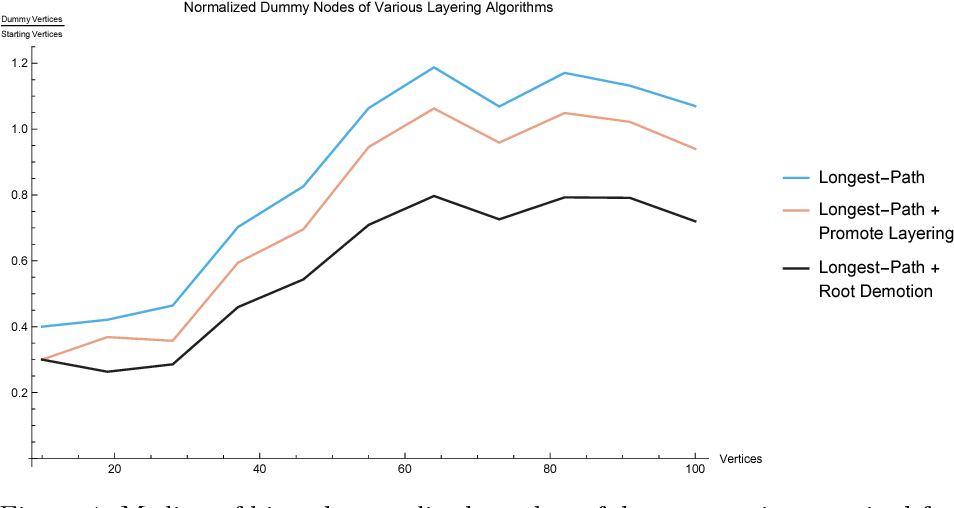
\includegraphics[width=0.6\linewidth]{./figures/dummy1.png}
	\caption{Dummy figure 1}%
	\label{fig:dummy1}
\end{figure}

\noindent Here are some citations \cite{einstein, latexcompanion}, and another 
example of display math \cite{knuthwebsite}:

\begin{table}[tb]
\centering
\caption{Dummy table}
\label{tab:dummy_tab}
\begin{tabular}{ |p{3cm}||p{3cm}|p{3cm}|p{3cm}|  }
 \hline
 \multicolumn{4}{|c|}{Country List} \\
 \hline
 Country Name     or Area Name& ISO ALPHA 2 Code &ISO ALPHA 3 Code&ISO numeric Code\\
 \hline
 Afghanistan   & AF    &AFG&   004\\
 Aland Islands&   AX  & ALA   &248\\
 Albania &AL & ALB&  008\\
 Algeria    &DZ & DZA&  012\\
 American Samoa&   AS  & ASM&016\\
 Andorra& AD  & AND   &020\\
 Angola& AO  & AGO&024\\
 \hline
\end{tabular} 
\end{table}

\begin{equation}
	\int_{-\infty}^\infty e^{-x^2} \dd x = \sqrt{\pi}
\end{equation}

Finally we have some code: \texttt{This is a demo of mono font}, and some
Sans Serif font: \textsf{Sans Serif}.


\chapter{Introduction}
\label{c:intro}

\lipsum[1-3]

\section{Intro 1}%
\label{sec:intro_1}

\lipsum[4]





\appendix

\backmatter

% add Bibliography to TOC
\phantomsection
\addcontentsline{toc}{chapter}{\bibname}

% Your bibliography goes here
\printbibliography

\end{document}
